
\documentclass[journal,10pt]{IEEEtran}
\usepackage{amsmath,amssymb,mathtools}
\usepackage{booktabs,array,tabularx,multirow}
\usepackage{graphicx}
\usepackage{xcolor}
\usepackage{enumitem}
\usepackage[hidelinks]{hyperref}
\usepackage{xurl}
\usepackage{tikz}
\usetikzlibrary{arrows.meta,positioning,fit,calc,shapes.geometric,backgrounds}
\usepackage{pgfplots}
\pgfplotsset{compat=1.18}
\usepackage{microtype}
\newcommand{\R}{\mathbb{R}}
\newcommand{\E}{\mathbb{E}}
\newcommand{\one}{\mathbf{1}}
\newcommand{\argmax}{\operatorname*{arg\,max}}
\newcommand{\argmin}{\operatorname*{arg\,min}}
\definecolor{nyuviolet}{RGB}{87,6,140}
\definecolor{deepblue}{RGB}{35,65,120}
\definecolor{darkgreen}{RGB}{25,110,70}
\tikzset{layer/.style={rectangle, rounded corners=3pt, draw=nyuviolet!75, very thick, fill=nyuviolet!6, align=center, minimum height=0.78cm, text width=2.75cm}, optbox/.style={rectangle, rounded corners=2pt, draw=deepblue!70, thick, fill=deepblue!5, align=center, minimum height=0.65cm, text width=3.1cm}, arrow/.style={-{Latex[length=2.5mm]}, thick, draw=black!65}, heatcell/.style={rectangle, minimum width=3.15cm, minimum height=0.70cm, draw=white, line width=0.9pt, font=\small\bfseries, align=center}}
\title{Portfolio Allocation as Layered System Optimization: Mathematical Modeling, Control Decomposition, and Empirical Evaluation}
\author{Ashesh~Kaji,~\IEEEmembership{Student,~New~York~University}%
\thanks{Ashesh Kaji is with New York University. Email: ask9184@nyu.edu.}}
\begin{document}
\maketitle
\begin{abstract}
This paper models portfolio allocation as a layered system optimization problem rather than a collection of isolated backtests. The study frames allocation as a sequential stochastic control problem incorporating discrete universe and screen decisions, continuous portfolio weights, transaction-cost control effort, and a learned meta-controller. The mathematical foundation relies on the Markowitz convex mean--variance program, extended through turnover-regularized optimal control, cardinality-constrained screening, online model selection, and policy-gradient reinforcement learning. Evaluated on liquid U.S. equity candidate universes of increasing breadth, the central finding is that the optimal control stack is not invariant: a top-100 candidate set favors a 21-day momentum screen followed by equal weighting; a top-250 set favors low-volatility screening with equal weighting; and a top-500 set favors volatility-adjusted momentum with short-horizon rank-and-hold weighting. Furthermore, a policy-gradient router over these arms recovers stable policies but does not strictly dominate a trailing-window adaptive rule, illustrating the tradeoffs between optimization complexity and realized value.
\end{abstract}
\begin{IEEEkeywords}
Portfolio optimization, stochastic control, cardinality-constrained optimization, online learning, reinforcement learning, transaction costs, walk-forward validation.
\end{IEEEkeywords}
\section{Motivation: Portfolio Allocation as a Sequential Control Problem}
The classical convex portfolio optimization problem seeks to estimate expected returns $\mu\in\R^n$ and covariance $\Sigma\succeq0$, and subsequently solve:
\begin{equation}
\begin{aligned}
\max_{w\in\R^n}\quad & \mu^\top w - \lambda w^\top \Sigma w\\
\text{s.t.}\quad & \one^\top w = 1,\qquad w\ge 0.
\end{aligned}
\label{eq:markowitz}
\end{equation}
While Equation~\ref{eq:markowitz} provides a foundational theoretical baseline as a convex quadratic program on the simplex, it is insufficient as a standalone model for live allocation systems. In practice, a portfolio controller must repeatedly solve a decision problem under uncertainty, update its active set, trade off exploitation against turnover, and adapt when the opportunity set changes.

The study therefore treats portfolio allocation as a closed-loop system. At each rebalance time $t$, the system observes market information $\mathcal{F}_t$, chooses a candidate universe $\mathcal{U}_t$, applies a screen $S_t$, chooses a weighting controller $C_t$, executes a portfolio $w_t$, and observes net reward after transaction costs. The resulting problem combines four optimization types:
\begin{enumerate}[leftmargin=1.5em]
    \item \textbf{Convex optimization:} continuous weight selection under risk and turnover penalties.
    \item \textbf{Combinatorial optimization:} cardinality-constrained subset selection over candidate securities.
    \item \textbf{Sequential control:} repeated portfolio adjustment under path-dependent transaction costs.
    \item \textbf{Online learning / reinforcement learning:} adaptive routing among screen/controller arms.
\end{enumerate}
The purpose of the final experiment is to determine which layer is doing useful work and when extra optimization complexity is justified.

\section{From Static Convex Optimization to Dynamic Control}
\subsection{Single-period convex model}
The Markowitz problem in Equation~\eqref{eq:markowitz} is convex after converting the maximization into minimization:
\begin{equation}
\min_{w\in\Delta_n}\; \lambda w^\top \Sigma w - \mu^\top w, \qquad \Delta_n=\{w:\one^\top w=1,\; w\ge0\}.
\end{equation}
It provides a clean language for risk aversion and diversification. The Lagrangian for the equality-constrained, unconstrained-sign version is
\begin{equation}
\mathcal{L}(w,\eta)=\lambda w^\top\Sigma w-\mu^\top w + \eta(\one^\top w-1),
\end{equation}
with first-order condition
\begin{equation}
2\lambda \Sigma w - \mu + \eta\one =0.
\end{equation}
This condition shows the central optimization tradeoff: weights tilt toward expected return only insofar as covariance-scaled risk permits. However, the empirical project repeatedly showed that estimating $\mu$ and $\Sigma$ is only one part of the decision. A controller can fail not because the convex program is badly solved, but because the universe or active set is not aligned with the signal being optimized.

\subsection{Turnover as control effort}
The first operational extension is to add trading friction. Let $w_{t^-}$ be the portfolio before rebalancing and $w_t$ the target portfolio. A proportional transaction-cost model is
\begin{equation}
\text{TC}_t = \kappa \lVert w_t-w_{t^-}\rVert_1,
\end{equation}
where $\kappa$ is the one-way cost rate. Let $\alpha_t\in\R^n$ denote the estimated conditional expected return vector at time $t$ (e.g., a trailing mean, momentum signal, or factor-based forecast). The corresponding turnover-regularized convex controller is
\begin{equation}
\begin{aligned}
\max_{w_t\in\Delta_n}\quad & \alpha_t^\top w_t - \lambda w_t^\top\widehat{\Sigma}_t w_t - \kappa\lVert w_t-w_{t^-}\rVert_1.
\end{aligned}
\label{eq:turnover_convex}
\end{equation}
Equation~\eqref{eq:turnover_convex} connects directly to dynamic trading models with transaction costs: the current position becomes part of the state, and turnover becomes control effort. Even when a rank-based controller rather than a full convex QP is used, the same control-cost logic remains central because high-churn rank-and-hold policies lose more to friction.

\subsection{Sequential objective}
The live problem is finite-horizon stochastic optimal control:
\begin{equation}
\max_{\pi}\; \E_\pi\left[\sum_{t=0}^{T-1}\delta^t\left(w_t^\top r_{t+1}-\kappa\lVert w_t-w_{t^-}\rVert_1-\rho\,\mathcal{R}(w_t,\mathcal{F}_t)\right)\right],
\label{eq:sequential_objective}
\end{equation}
where $w_t$ is the post-trade portfolio, $w_{t^-}$ is the pre-trade portfolio, $r_{t+1}$ is the next-period return vector, $\kappa$ is the transaction-cost coefficient, $\rho$ is a risk-penalty coefficient, $\pi$ maps observed state to actions, $\delta$ is a discount factor, and $\mathcal{R}$ is a risk or instability penalty (not used in the empirical evaluation, which relies on the turnover term alone to penalize control effort). If the transition model were known, the corresponding Bellman recursion could be written by setting $x_t=(\mathcal{F}_t,w_{t^-})$, $a_t=w_t$, and
\begin{equation}
g(x_t,a_t)=\E\!\left[w_t^\top r_{t+1}\mid\mathcal{F}_t\right]-\kappa\lVert w_t-w_{t^-}\rVert_1-\rho\,\mathcal{R}(w_t,\mathcal{F}_t),
\end{equation}
so that
\begin{equation}
V_t(x_t)=\max_{a_t\in\mathcal{A}(x_t)}\left\{g(x_t,a_t)+\delta\E[V_{t+1}(x_{t+1})\mid x_t,a_t]\right\}.
\end{equation}
Here $\mathcal{A}(x_t)$ encodes the admissible portfolio simplex, eligibility, leverage, and turnover constraints, with terminal value normalized as $V_T(x_T)=0$ for the finite-horizon evaluation used in the backtests.
The implemented study approximates this ideal control problem through interpretable policy classes: screens, rank-and-hold rules, equal weighting, and learned routing. The empirical question is not whether the theoretical Bellman equation can be solved exactly; it is whether decomposition into tractable subproblems produces better and more interpretable allocation decisions.

\section{Layered Mathematical Formulation}
\subsection{Bilevel mixed discrete-continuous view}
Let $b\in\{100,250,500\}$ index candidate-universe breadth, $j\in\mathcal{J}$ index a screen, and $k\in\mathcal{K}$ index a weighting controller. The full model-selection problem can be written as
\begin{equation}
\begin{aligned}
\max_{b,j,k}\quad & \frac{\widehat{\mu}_{b,j,k}}{\widehat{\sigma}_{b,j,k}} - \phi\,\widehat{\text{DD}}_{b,j,k} - \psi\,\widehat{\text{TO}}_{b,j,k}\\
\text{s.t.}\quad & H_{b,j}(t)=S_j(\mathcal{U}_b(t),\mathcal{F}_t),\\
& w_t=C_k(H_{b,j}(t),\mathcal{F}_t,w_{t^-}),\\
& |H_{b,j}(t)|\le K_{\max},\qquad w_t\in\Delta_{|H_{b,j}(t)|}.
\end{aligned}
\label{eq:bilevel_stack}
\end{equation}
Here $\widehat{\mu}_{b,j,k}$, $\widehat{\sigma}_{b,j,k}$, $\widehat{\text{DD}}_{b,j,k}$, and $\widehat{\text{TO}}_{b,j,k}$ are walk-forward estimates of mean return, volatility, drawdown, and turnover for the stack $(b,j,k)$. This is not a single convex program. It is a mixed discrete-continuous model-selection problem with lower-level portfolio maps embedded in $C_k$. The empirical design makes it tractable by enumerating a disciplined grid of $(b,j,k)$ arms, evaluating each arm out of sample, and then studying the performance surface.

\begin{figure*}[!t]
\centering
\resizebox{0.98\textwidth}{!}{%
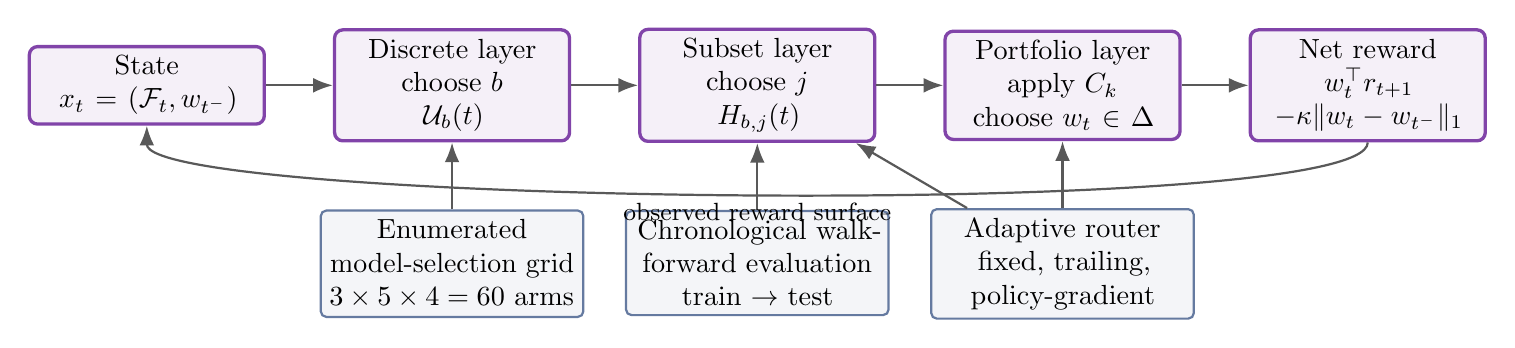
\begin{tikzpicture}[node distance=0.65cm and 0.85cm]
\node[layer] (state) {State\\$x_t=(\mathcal{F}_t,w_{t^-})$};
\node[layer, right=of state] (universe) {Discrete layer\\choose $b$\\$\mathcal{U}_b(t)$};
\node[layer, right=of universe] (screen) {Subset layer\\choose $j$\\$H_{b,j}(t)$};
\node[layer, right=of screen] (weights) {Portfolio layer\\apply $C_k$\\choose $w_t\in\Delta$};
\node[layer, right=of weights] (reward) {Net reward\\$w_t^\top r_{t+1}$\\$-\kappa\|w_t-w_{t^-}\|_1$};
\node[optbox, below=0.85cm of universe] (enumerate) {Enumerated model-selection grid\\$3\times5\times4=60$ arms};
\node[optbox, below=0.85cm of screen] (wf) {Chronological walk-forward evaluation\\train $\rightarrow$ test};
\node[optbox, below=0.85cm of weights] (router) {Adaptive router\\fixed, trailing, policy-gradient};
\draw[arrow] (state)--(universe);
\draw[arrow] (universe)--(screen);
\draw[arrow] (screen)--(weights);
\draw[arrow] (weights)--(reward);
\draw[arrow] (enumerate)--(universe);
\draw[arrow] (wf)--(screen);
\draw[arrow] (router)--(screen);
\draw[arrow] (router)--(weights);
\draw[arrow] (reward.south) .. controls +(0,-1.0) and +(0,-1.0) .. node[below,font=\small]{observed reward surface} (state.south);
\end{tikzpicture}}
\caption{Optimization decomposition used in the study. A difficult mixed discrete-continuous sequential problem is decomposed into enumerated universe/screen/controller arms, walk-forward evaluation, and an adaptive routing layer.}
\label{fig:decomposition}
\end{figure*}

\subsection{Screens as constrained projections}
Each screen is a set-valued map from the candidate universe into a smaller active set:
\begin{equation}
S_j:\left(\mathcal{U}_b(t),\mathcal{F}_t\right)\mapsto H_{b,j}(t),\qquad |H_{b,j}(t)|\le K_{\max}.
\end{equation}
For a score $q_i(t)$, the top-$K$ screen solves the cardinality problem
\begin{equation}
\max_{z\in\{0,1\}^{|\mathcal{U}|}}\; \sum_{i\in\mathcal{U}} q_i(t)z_i
\quad\text{s.t.}\quad \sum_i z_i\le K.
\label{eq:topk}
\end{equation}
The five score functions tested are
\begin{align}
q_i^{\text{mom},\tau}(t) &= P_i(t)/P_i(t-\tau)-1,\\
q_i^{\text{vam},\tau}(t) &= \frac{P_i(t)/P_i(t-\tau)-1}{\widehat{\sigma}_{i,\tau}(t)+\epsilon},\\
q_i^{\text{lowvol},\tau}(t) &= -\widehat{\sigma}_{i,\tau}(t),\\
q_i^{\text{cluster}}(t) &= q_i^{\text{mom},63}(t)\quad\text{with per-cluster selection caps}.
\end{align}
This is where a major system-optimization insight enters the project: screening is not data cleaning. It is a discrete optimization layer that changes the feasible set available to every downstream controller.

\subsection{Weighting controllers as restricted policy classes}
After screening, the controller chooses weights on the active set $H_t$. Equal weighting is the minimum-estimation controller:
\begin{equation}
w_{i,t}=\frac{1}{|H_t|}\mathbf{1}\{i\in H_t\}.
\end{equation}
Rank-and-hold is another cardinality-constrained policy, now inside the screened set:
\begin{equation}
w_{i,t}=\frac{1}{k}\mathbf{1}\left\{i\in\operatorname{TopK}_{\ell\in H_t}\left(P_\ell(t)/P_\ell(t-\tau)-1\right)\right\}.
\label{eq:rank_hold}
\end{equation}
Although Equation~\eqref{eq:rank_hold} is simpler than a full quadratic program, it is still an optimization rule: it solves a top-$k$ linear ranking objective over the screened active set. The final study compares whether this extra active layer is worth its turnover cost after screening has already concentrated the universe.

\section{Learning and Meta-Control Formulation}
\subsection{Model selection as an online expert problem}
Let each screen/controller pair be an arm $a\in\mathcal{A}$ with realized reward $R_t(a)$ in walk-forward period $t$. A non-learning model-selection baseline chooses
\begin{equation}
a^{\text{train}}=\argmax_{a\in\mathcal{A}}\sum_{t\in\mathcal{T}_{\text{train}}}R_t(a)
\end{equation}
and holds that arm in the test period. The trailing-window router chooses
\begin{equation}
a_t^{\text{trail}}=\argmax_{a\in\mathcal{A}}\sum_{s=t-L}^{t-1}R_s(a),
\end{equation}
which is an online adaptive rule. This comparator is important because any learned method must beat simple, transparent online optimization before it can be considered practically useful.

\subsection{Policy-gradient router}
The reinforcement-learning router treats the arm-selection problem as a finite-action Markov decision process. The state $s_t$ contains time features, scope identity, trailing rewards, and the most recent reward vector. The policy is a softmax over arm logits:
\begin{equation}
\pi_\theta(a\mid s_t)=\frac{\exp(f_\theta(s_t)_a)}{\sum_{a'\in\mathcal{A}}\exp(f_\theta(s_t)_{a'})}.
\end{equation}
The reward is next-period net reward minus a switching penalty:
\begin{equation}
r_t^{\text{router}}=R_t(a_t)-\xi\mathbf{1}\{a_t\ne a_{t-1}\}.
\end{equation}
The policy-gradient update estimates
\begin{equation}
\nabla_\theta J(\theta)=\E_\pi\left[\sum_t (G_t-b_t)\nabla_\theta\log\pi_\theta(a_t\mid s_t)\right],
\label{eq:policy_gradient}
\end{equation}
where $G_t$ is a return-to-go and $b_t$ is a variance-reduction baseline. The important methodological choice is that reinforcement learning is not asked to learn raw portfolio weights from scratch. It is placed at the system level, where the action space consists of interpretable optimization stacks.

\section{Experimental Protocol as Optimization Evidence}
The final empirical matrix uses three universe scopes, five screens, and four weighting controllers, producing $3\times5\times4=60$ primary arms at the 10 basis point cost slice. Each arm is evaluated through chronology-respecting walk-forward splits: screen membership is computed using only information available through the training end date, and performance is measured on the subsequent evaluation interval. This is the empirical analogue of out-of-sample control evaluation.

\begin{table*}[!t]
\centering
\caption{Layer map of the optimization decomposition and its empirical instantiations.}
\label{tab:layer_map}
\small
\begin{tabularx}{\textwidth}{p{2.6cm}p{3.8cm}X}
\toprule
Layer & Mathematical role & Implementation in final study\\
\midrule
Universe breadth & Discrete state/action defining candidate feasible set & Top-100, top-250, and top-500 liquid-equity candidate scopes\\
Screen & Cardinality-constrained subset optimization & Momentum, volatility-adjusted momentum, low-volatility, cluster-capped momentum top-10 screens\\
Weighting & Continuous or restricted portfolio policy on simplex & Equal weight and 21/63/126-day rank-and-hold top-5 controllers\\
Trading friction & Control effort / path dependence & Net reward subtracts proportional turnover cost at 10 bps primary slice\\
Routing & Online model selection / MDP policy & Train-selected fixed arm, trailing-window router, random router, policy-gradient router, oracle bounds\\
Validation & Out-of-sample control evaluation & Chronological walk-forward splits, all-trials ledger, model-selection ledger, multiple-comparison diagnostic\\
\bottomrule
\end{tabularx}
\end{table*}

\section{Optimization Results}
\subsection{Main solution stacks}
The strongest empirical evidence that the layered model matters is that the selected solution stack changes with universe breadth.
\begin{table*}[!t]
\centering
\caption{Best screen/controller stack by candidate-universe breadth. Values are mean walk-forward metrics at 10 bps transaction cost.}
\label{tab:winners_math}
\small
\resizebox{\textwidth}{!}{%
\begin{tabular}{lllrrrrr}
\toprule
Universe & Discrete screen solution & Weighting solution & Splits & Ann. ret. & Ann. vol. & Sharpe & Worst DD\\
\midrule
Top-100 & 21-day momentum top 10 & Equal weight & 22 & 20.4\% & 20.2\% & 1.474 & -44.9\%\\
Top-250 & 63-day low-volatility top 10 & Equal weight & 11 & 11.2\% & 14.1\% & 0.859 & -10.5\%\\
Top-500 & Vol.-adjusted 63-day momentum top 10 & 21-day rank-and-hold & 9 & 35.1\% & 20.8\% & 1.756 & -15.5\%\\
\bottomrule
\end{tabular}%
}
\end{table*}
The optimization interpretation is direct. If the universe is narrow, screening already performs most of the selection and equal weighting is an adequate solution on the resulting simplex. In the broadest universe, the feasible set contains enough cross-sectional dispersion that a second ranking optimization inside the screened set improves risk-adjusted performance. In the intermediate universe, low-volatility screening dominates, suggesting that the best solution is to reduce noise rather than chase momentum.

\subsection{Screen layer: objective functions matter}
\begin{figure*}[!t]
\centering
\resizebox{0.98\textwidth}{!}{%
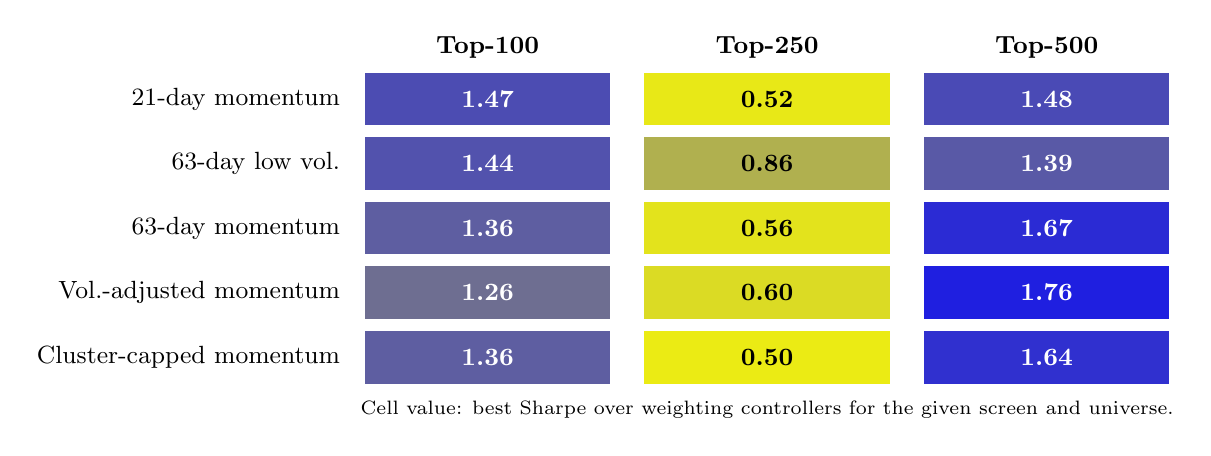
\begin{tikzpicture}
\node[heatcell, fill=blue!70!yellow, text=white] at (0.0,0.0) {1.47};
\node[heatcell, fill=blue!9!yellow, text=black] at (3.55,0.0) {0.52};
\node[heatcell, fill=blue!71!yellow, text=white] at (7.10,0.0) {1.48};
\node[heatcell, fill=blue!68!yellow, text=white] at (0.0,-0.82) {1.44};
\node[heatcell, fill=blue!31!yellow, text=black] at (3.55,-0.82) {0.86};
\node[heatcell, fill=blue!65!yellow, text=white] at (7.10,-0.82) {1.39};
\node[heatcell, fill=blue!63!yellow, text=white] at (0.0,-1.64) {1.36};
\node[heatcell, fill=blue!11!yellow, text=black] at (3.55,-1.64) {0.56};
\node[heatcell, fill=blue!83!yellow, text=white] at (7.10,-1.64) {1.67};
\node[heatcell, fill=blue!57!yellow, text=white] at (0.0,-2.46) {1.26};
\node[heatcell, fill=blue!14!yellow, text=black] at (3.55,-2.46) {0.60};
\node[heatcell, fill=blue!88!yellow, text=white] at (7.10,-2.46) {1.76};
\node[heatcell, fill=blue!63!yellow, text=white] at (0.0,-3.28) {1.36};
\node[heatcell, fill=blue!8!yellow, text=black] at (3.55,-3.28) {0.50};
\node[heatcell, fill=blue!81!yellow, text=white] at (7.10,-3.28) {1.64};
\foreach \j/\name in {0/{Top-100},1/{Top-250},2/{Top-500}} {\node[font=\small\bfseries, align=center] at (\j*3.55,0.65) {\name};}
\foreach \i/\name in {0/{21-day momentum},1/{63-day low vol.},2/{63-day momentum},3/{Vol.-adjusted momentum},4/{Cluster-capped momentum}} {\node[font=\small, anchor=east, align=right] at (-1.75,-\i*0.82) {\name};}
\node[font=\scriptsize, align=center] at (3.55,-3.95) {Cell value: best Sharpe over weighting controllers for the given screen and universe.};
\end{tikzpicture}}
\caption{Screen objective functions define different feasible active sets. The heatmap shows that the best screening objective changes by universe breadth.}
\label{fig:screen_heatmap_math}
\end{figure*}
Figure~\ref{fig:screen_heatmap_math} is the most compact visual evidence that the screen is an optimization layer. The top-250 universe is weak across most momentum screens, but improves under the low-volatility objective. The top-500 universe rewards volatility-adjusted and medium-horizon momentum objectives. Thus, the screen objective changes the feasible set in a way that can dominate the weighting rule.

\subsection{Weighting layer: when extra control effort pays}
Averaging over screens, equal weighting has the best mean Sharpe in the top-100 and top-250 scopes, while 21-day rank-and-hold has the best mean Sharpe in the top-500 scope. This is a system-level cost-benefit result. Extra optimization effort is not universally valuable; it is valuable when the upstream feasible set is broad enough to contain exploitable dispersion.
\begin{table*}[!t]
\centering
\caption{Controller ablation: best weighting rule averaged over screens.}
\label{tab:controller_ablation_math}
\small
\resizebox{\textwidth}{!}{%
\begin{tabular}{llrrp{5.0cm}}
\toprule
Universe & Best controller by average screen Sharpe & Mean Sharpe & Best Sharpe & Interpretation\\
\midrule
Top-100 & Equal weight & 1.380 & 1.474 & screen does most selection\\
Top-250 & Equal weight & 0.572 & 0.859 & risk filtering beats active ranking\\
Top-500 & 21-day rank-and-hold & 1.433 & 1.756 & breadth justifies second control layer\\
\bottomrule
\end{tabular}
}
\end{table*}
The turnover diagnostics support the same conclusion. Equal weight has essentially zero rebalance turnover after screen membership is fixed, while rank-and-hold rules introduce substantial turnover. When active ranking does not add enough signal, the turnover penalty makes the simpler controller superior.

\subsection{Model-selection risk and multiple comparisons}
Because each universe evaluates 20 screen/controller arms, a winning Sharpe must be interpreted as a selected maximum over many trials:
\begin{equation}
\widehat{a} = \argmax_{a\in\mathcal{A}} \widehat{\text{SR}}(a).
\end{equation}
The study therefore reports the winner gap against the second-best arm, supplemented by a block-bootstrap procedure (2,000 resamples of walk-forward splits) to assess the stability of the selected winner. The bootstrap resamples the split-level Sharpe ratios with replacement, preserving the time structure of the walk-forward folds, and recomputes the best arm and winner gap in each resample.

\begin{table*}[!t]
\centering
\caption{Model-selection risk diagnostic with block-bootstrap 95\% confidence intervals. The bootstrap resamples walk-forward splits to assess winner stability; a gap whose CI includes zero indicates that the best and second-best arms are not reliably ordered.}
\label{tab:selection_risk_math}
\small
\begin{tabular}{lrrrrrrc}
\toprule
Universe & Arms & Splits & Best Sharpe & Second Sharpe & Gap & 95\% CI & Win.\ rate\\
\midrule
Top-100 & 20 & 22 & 1.474 & 1.440 & 0.034 & [0.000, 0.294] & 35.7\%\\
Top-250 & 20 & 11 & 0.859 & 0.755 & 0.104 & [0.004, 0.545] & 33.8\%\\
Top-500 & 20 & 9 & 1.756 & 1.666 & 0.090 & [0.000, 0.366] & 36.4\%\\
\bottomrule
\end{tabular}
\end{table*}
The bootstrap reveals that winner stability is low: the point-estimate best arm is selected in approximately one-third of bootstrap samples across all three universes. Moreover, two of three winner-gap confidence intervals include zero. This fragility is expected given 9--22 walk-forward splits and 20 arms per universe. The results should therefore be interpreted as mechanism evidence — documenting how the performance surface changes across layers — rather than as a claim that any specific arm is the uniquely optimal choice.

\section{Reinforcement Learning as System-Level Optimization}
The learned router is placed as a meta-controller over already-interpretable optimization arms: it is not a black-box replacement for portfolio theory, but a learned model-selection policy in a structured control system.

\begin{table*}[!t]
\centering
\caption{Integrated policy-gradient router results. Rewards are cumulative test-period rewards at the 10 bps cost slice; RL values are mean $\pm$ standard deviation over seven seeds for the best configuration.}
\label{tab:rl_math}
\scriptsize
\begin{tabular}{lrrrrrrrr}
\toprule
Scope & Test periods & RL & Train-fixed & Trailing & Random & Oracle & RL--fixed & RL--trailing\\
\midrule
Combined & 14 & 1.213 $\pm$ 0.063 & 1.134 & 1.543 & 1.276 & 2.586 & 0.079 & -0.330\\
Top-100 & 8 & 0.823 $\pm$ 0.011 & 0.827 & 0.475 & 0.657 & 1.355 & -0.004 & 0.348\\
Top-250 & 5 & 0.280 $\pm$ 0.068 & 0.305 & 0.306 & 0.296 & 0.764 & -0.026 & -0.026\\
Top-500 & 4 & 0.371 $\pm$ 0.000 & 0.371 & 0.566 & 0.525 & 0.932 & 0.000 & -0.196\\
\bottomrule
\end{tabular}
\end{table*}
The policy-gradient router improves over the train-selected fixed arm in the combined panel and learns stable selections, but it does not dominate the trailing-window router. In optimization terms, the learned policy class and state representation are sufficient to recover some structure in the reward surface, but not sufficient to beat a low-complexity online optimizer that directly exploits recent realized rewards.

\begin{figure*}[!t]
\centering
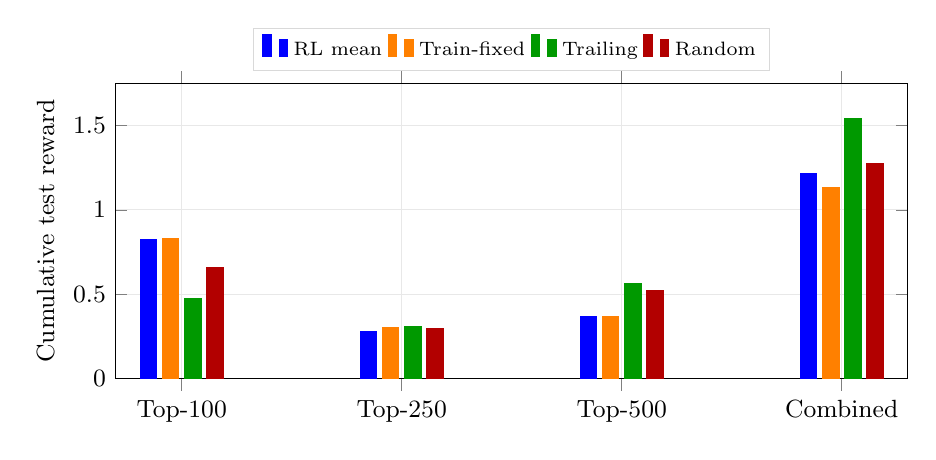
\begin{tikzpicture}
\begin{axis}[ybar,bar width=6pt,width=0.96\textwidth,height=0.44\textwidth,ylabel={Cumulative test reward},symbolic x coords={Top-100,Top-250,Top-500,Combined},xtick=data,ymin=0,ymax=1.75,grid=major,grid style={gray!18},legend style={at={(0.5,1.04)}, anchor=south, legend columns=4, font=\scriptsize, draw=gray!30},tick label style={font=\small},label style={font=\small}]
\addplot+[ybar, fill=blue, draw=blue] coordinates {(Top-100,0.823) (Top-250,0.280) (Top-500,0.371) (Combined,1.213)};
\addlegendentry{RL mean}
\addplot+[ybar, fill=orange, draw=orange] coordinates {(Top-100,0.827) (Top-250,0.305) (Top-500,0.371) (Combined,1.134)};
\addlegendentry{Train-fixed}
\addplot+[ybar, fill=green!60!black, draw=green!60!black] coordinates {(Top-100,0.475) (Top-250,0.306) (Top-500,0.566) (Combined,1.543)};
\addlegendentry{Trailing}
\addplot+[ybar, fill=red!70!black, draw=red!70!black] coordinates {(Top-100,0.657) (Top-250,0.296) (Top-500,0.525) (Combined,1.276)};
\addlegendentry{Random}
\end{axis}
\end{tikzpicture}
\caption{Adaptive model-selection comparison. The trailing-window rule is a strong online optimization baseline; the learned router is informative but not yet dominant.}
\label{fig:rl_math_bar}
\end{figure*}

\section{Limitations and Next Mathematical Step}
The main limitations are also optimization limitations. First, the candidate universes are not fully point-in-time, so the feasible sets $\mathcal{U}_b(t)$ are only approximations to investable historical universes. Second, the screen/controller grid is finite; it approximates the bilevel problem but does not solve the full mixed-integer program in Equation~\eqref{eq:bilevel_stack}. Third, the RL router has few independent test periods per scope, so policy-gradient results should be treated as exploratory. Fourth, market impact is modeled as proportional turnover rather than a nonlinear function of order size and liquidity.

The next rigorous step is not another broad sweep. It is to build point-in-time universe membership and rerun the layered system with more independent walk-forward episodes. Mathematically, this would improve the fidelity of the feasible set $\mathcal{U}_b(t)$ and provide enough samples to evaluate whether learned routing approximates the online model-selection optimum better than simple trailing-window selection.


\section{Implementation and Numerical Procedure}
The computational engine used in the study is organized around three objects: price panels, decision rules, and walk-forward ledgers. A price panel is a date-by-asset matrix of adjusted close prices, from which returns, trailing momentum, realized volatility, and correlation descriptors are computed. A decision rule is a deterministic or learned map from past information to an active set and target weights. A ledger is a record of every split, arm, cost slice, gross return, net return, drawdown, and selected configuration. The ledger design matters because it prevents the final report from depending only on selected winners; every arm in the primary grid is preserved for ablation and multiple-comparison diagnostics.

The primary numerical procedure is as follows. First, define the candidate universe breadth $b$. Second, for each training window, compute all screen scores using only data available through the training end date. Third, select a top-$K$ active set for each screen. Fourth, apply each weighting controller to produce target weights on the active set. Fifth, evaluate the resulting portfolio over the following test window, subtracting proportional transaction costs from turnover. Sixth, write both arm-level and split-level outputs so that later analysis can average by universe, screen, controller, and time period. This procedure is simple enough to audit but rich enough to expose the interactions between universe breadth and controller complexity.

The learned router uses the same saved reward matrix rather than a separate hidden simulation. This design choice reduces the risk that reinforcement learning receives a privileged evaluation environment. The state contains recent reward history and scope information; the action is a discrete choice of screen/controller arm; the reward is the next realized net return minus a switching penalty. The policy-gradient update is therefore a meta-control algorithm over already interpretable portfolio policies. The learned policy is judged against train-selected fixed routing, trailing-window routing, random routing, and an oracle upper bound. This makes the RL component a proper numerical example of adaptive system optimization rather than an ungrounded black-box add-on.

\section{Discussion}
The most important evidence of depth is that the study follows one motivating anomaly---the dependence of controller performance on universe breadth---until it becomes a mechanism-level claim. A broad benchmark would merely list many strategies. This paper instead asks why the same weighting controller is not best across candidate sets, and it separates three possible explanations: the screen objective changes the feasible set, the weighting rule changes the exploitation of that set, and the router changes the timing of model selection.

The results support a practical hierarchy. In narrow candidate sets, most useful selection occurs before the weighting problem; once the active set is constructed, equal weighting is a robust low-estimation solution. In broad candidate sets, the active set retains enough cross-sectional dispersion that a second ranking layer can add value despite turnover. In the intermediate candidate set, the best result comes from low-volatility filtering rather than momentum chasing, suggesting that a universe can be broad enough to introduce noise but not broad enough to reliably reward additional active selection. This middle-case result is analytically significant because it prevents the conclusion from becoming a monotone ``larger universe is always better'' story.

The routing results add another layer of interpretation. The learned router is not a failure merely because it does not dominate trailing-window selection. Its non-dominance is itself informative: a simple online optimizer that reacts directly to recent realized rewards is a strong baseline in this finite-sample setting. The learned router recovers stable preferences and improves over train-fixed selection in the combined panel, but the current state representation and number of independent episodes are insufficient to justify deployable superiority. The architecture is promising, while the evidence is not yet strong enough for an operational claim.


\section{Additional Diagnostics: Robustness, Costs, and Selection Bias}
A key reason the project is framed as system optimization rather than as strategy search is that a backtest winner can be misleading when it is selected from a large grid. The primary grid has 60 arms at the canonical transaction-cost slice, and additional cost-sensitivity slices are used diagnostically. Therefore, the empirical question is not simply which arm has the largest realized Sharpe ratio. The more relevant question is whether the same mechanism appears after decomposing the surface by universe, screen, controller, cost, and fold.

The first diagnostic is the stability of the selected winner assessed via block-bootstrap (Table~\ref{tab:selection_risk_math}). The winner gap confidence intervals include zero for the top-100 and top-500 universes, and the point-estimate best arm is selected in only 33--37\% of bootstrap samples. The results should therefore be interpreted as mechanism evidence — documenting how the performance surface changes across layers — rather than as a claim that any specific arm is the uniquely optimal choice.

The second diagnostic is cost sensitivity. The same winning stack is selected at 0, 10, and 25 basis point cost levels in all three universes, indicating that the winner ordering is not an artifact of the cost parameter. In the top-500 universe, the high-turnover rank-and-hold winner sees its Sharpe decline from 1.814 to 1.669 as costs increase, but it remains the best arm — consistent with the interpretation that breadth creates enough dispersion to reward active rebalancing even after moderate friction.

The third diagnostic is the distinction between gross and net performance. A controller that frequently changes holdings must overcome its own control effort. This is the practical meaning of the turnover penalty in the objective. Equal weighting has low implementation complexity and tends to trade mainly when screen membership changes. Rank-and-hold controllers add an additional active selection layer and therefore can generate higher turnover. The top-500 result is interesting because this extra control layer appears to pay for itself. The top-100 and top-250 results are equally important because they show the opposite: once the screen has performed the main selection, additional ranking can be unnecessary or harmful.

The fourth diagnostic is subperiod behavior. Walk-forward validation does not eliminate nonstationarity, but it forces the controller to earn returns in test intervals that follow the estimation interval. This is more appropriate than a full-sample optimization because portfolio controllers are deployed sequentially. The saved split-level ledger makes it possible to ask whether an arm wins because of one exceptional fold or because it has a more consistent distribution of split-level rewards. The current submission summarizes the mean surface and the primary winner gaps; future work should add confidence intervals or block-bootstrap intervals once the point-in-time universe construction increases the number of independent folds.

\section{Algorithmic Description}
For clarity, the core numerical experiment can be summarized in algorithmic form. Let $B$ be the set of candidate breadths, $J$ the set of screens, $K$ the set of weighting controllers, and $\mathcal{W}$ the set of chronological train/test splits. For each $b\in B$, a candidate price panel is formed. For each split $s\in\mathcal{W}$, all statistics are computed only on the training part of that split. For each screen $j\in J$, a score vector $q_j(t)$ is computed and the active set $H_{b,j}(t)$ is selected by a top-$K$ cardinality rule. For each controller $k\in K$, target weights are generated and evaluated over the test interval. Net reward is stored as the realized portfolio return minus the turnover cost. The output is a tensor indexed by universe, screen, controller, split, and cost slice.

\begin{table*}[!t]
\centering
\caption{Conceptual pseudocode for the walk-forward optimization experiment. The design records every tried arm rather than only the selected winner.}
\label{tab:pseudocode}
\small
\begin{tabularx}{\textwidth}{p{0.08\textwidth}X}
\toprule
Step & Operation \\
\midrule
1 & Choose candidate-universe breadth $b\in\{100,250,500\}$ and form the corresponding adjusted-close price panel.\\
2 & Generate chronological train/test splits; never use test-window observations to compute screens or controller statistics.\\
3 & For each screen $j$, compute scores such as momentum, volatility-adjusted momentum, low volatility, or cluster-capped momentum.\\
4 & Select active set $H_{b,j}(t)$ using a top-$K$ cardinality rule, making screening an explicit discrete optimization layer.\\
5 & For each weighting controller $k$, compute target weights on $H_{b,j}(t)$ using equal weighting or rank-and-hold selection.\\
6 & Evaluate net test reward $w_t^\top r_{t+1}-\kappa\|w_t-w_{t^-}\|_1$ and store return, volatility, Sharpe, drawdown, and turnover.\\
7 & Aggregate the full tensor by universe, screen, and controller; separately evaluate fixed, trailing-window, random, learned, and oracle routers.\\
\bottomrule
\end{tabularx}
\end{table*}

This algorithmic structure is deliberately modular. New screens can be added without changing the weighting layer. New controllers can be added without changing the universe construction. New routers can be trained on the same reward tensor, which makes learned routing comparable to transparent online baselines. The modularity is part of the contribution because it turns a broad project into an extensible numerical package for asking increasingly precise system-optimization questions.

\section{Why the Middle-Breadth Universe Matters}
The weakest empirical scope, the top-250 candidate set, is not a nuisance result to be hidden. It is one of the more useful findings because it shows that universe breadth does not have a monotone relationship with performance. A superficial conclusion might be that more stocks always create better selection opportunities. The results do not support that view. The top-250 universe is broad enough to introduce additional noise and dispersion, but in this experiment it does not provide as favorable a selection surface as the top-500 universe. Consequently, low-volatility filtering dominates momentum chasing in that scope.

This result motivates the next deep study. The first possibility is that the top-250 candidate set is structurally different: it may contain many names with unstable trends, higher idiosyncratic noise, or less persistent cross-sectional momentum. The second possibility is that the candidate construction is imperfect: symbol limits and current-constituent membership may create an artificial middle universe. The third possibility is that the evaluation sample is too small to distinguish persistent structure from period-specific noise. Each explanation leads to a concrete optimization experiment: compute structural descriptors, rebuild point-in-time membership, and add more independent walk-forward episodes.

The important academic point is that the study now has a falsifiable mechanism. If a future point-in-time top-250 universe remains weak and low-volatility-dominated, then the middle-breadth effect is likely structural. If the effect disappears after better membership construction, then the limitation was data engineering. If confidence intervals remain wide, then the correct conclusion is that the current sample cannot support scope-specific deployment. In all three cases, the research becomes deeper because the anomaly directs the next experiment.

\section{Future Research Program}
The next research step should be narrower and deeper rather than broader. The first priority is point-in-time universe membership. In the current experiment, candidate breadth is informative, but the universe definition is still approximate. A stronger version of the study would reconstruct eligible names at each historical date using membership, delisting, liquidity, and price-availability filters. This would transform $\mathcal{U}_b(t)$ from an approximate current-constituent set into a true time-varying feasible set. The main empirical question would then be whether the same stack ordering survives: momentum/equal-weight for narrow universes, low-volatility/equal-weight for the middle universe, and volatility-adjusted momentum/rank-and-hold for the broad universe.

A natural extension is to model crowding effects as interaction terms in the sequential objective, treating each strategy family as an agent in a non-cooperative game. The present paper provides the single-agent control substrate that such a multi-agent extension would require.

The second priority is descriptor-conditioned analysis. For each walk-forward training window, the study should compute average pairwise correlation, first principal-component share, cross-sectional dispersion, realized volatility, trend persistence, volatility-of-volatility, liquidity concentration, and turnover pressure. These descriptors would convert the qualitative claim that ``universe structure matters'' into a supervised prediction problem: given the structure of a candidate universe, predict which screen/controller family should be preferred. This is where the project can become practically useful. A portfolio researcher does not only want to know which controller won historically; the researcher wants a rule for deciding when to deploy each controller.

The third priority is a larger routing experiment. The current learned router is constrained by few independent test episodes. With more point-in-time folds and descriptor features, the router could be evaluated as a true contextual policy. The comparison set should remain strict: train-selected fixed selection, trailing-window routing, random routing, and oracle upper bounds. A learned model that cannot beat trailing-window routing should not be considered deployable, even if it has appealing architecture. Conversely, a learned router that beats trailing-window routing across independent folds would be a meaningful system-optimization result because it would show that the descriptor state contains predictive information beyond recent rewards.

The fourth priority is a richer cost model. The present proportional cost model is appropriate for controlled comparison, but real portfolio implementation depends on liquidity, order size, participation rate, and market impact. A more realistic objective would replace $\kappa\|w_t-w_{t^-}\|_1$ with a function such as $c_i|\Delta w_{i,t}|+m_i(\Delta w_{i,t})^2$, where $c_i$ captures spread-like linear costs and $m_i$ captures nonlinear impact. This would make universe selection even more central because the feasible set would no longer be defined only by return history; it would also be defined by tradability.

These extensions preserve the thesis while improving rigor. They do not require inventing a new story. They follow the strongest result of the current project: portfolio allocation is a layered control problem, and the practical value of optimization depends on knowing which layer is currently binding.

\section{Practical Takeaways}
The study produces several practical implications. First, optimize the opportunity set before over-engineering the optimizer: if the universe is poorly aligned with the signal, a more sophisticated weighting solver may only optimize noise. Second, treat screens as decision rules, not preprocessing — momentum, volatility-adjusted momentum, low-volatility filtering, and cluster-capped momentum each induce a different feasible portfolio problem. Third, keep equal weighting in the benchmark set; after screening, equal weighting can be a low-variance controller that avoids estimation error and turnover. Fourth, add active ranking only when the universe is broad enough to make the second selection layer worthwhile. Fifth, require any learned meta-controller to beat transparent adaptive baselines before treating it as a practical improvement.

These conclusions suggest an operational research workflow: characterize the candidate universe; choose a screen that matches its statistical structure; compare the simplest feasible weighting controller against more active alternatives; then evaluate whether adaptive routing adds value beyond a trailing-window rule. This workflow is more useful than searching for a single universally best portfolio algorithm.

\section{Conclusion}
This study provides evidence that, within the tested walk-forward design, the optimal portfolio allocation method is not a static weighting formula, but rather a dynamic stack comprising universe construction, screen objectives, weighting controllers, and optional routing. In a narrow top-100 universe, the optimal solution requires minimal estimation: momentum screening paired with equal weighting. In a top-250 universe, risk filtering becomes the dominant optimization. As breadth expands to a top-500 universe, the increased cross-sectional dispersion justifies the complexity of volatility-adjusted momentum combined with short-horizon rank-and-hold weighting. The learned router confirms that the hierarchy is learnable, but also demonstrates that a transparent trailing-window optimizer remains a difficult baseline. Once portfolio allocation is modeled as a mixed discrete-continuous sequential control problem, the analysis shifts from searching for a single best trading rule to determining where optimization should be applied: to the feasible set, to the weights, to the control cost, or to the routing policy.



\appendices
\section{Controller and Screen Grid}
The primary grid contains three candidate-universe breadth levels, five screen rules, and four weighting controllers. The screen rules are 21-day momentum top 10, 63-day momentum top 10, 63-day volatility-adjusted momentum top 10, 63-day low-volatility top 10, and 63-day cluster-capped 63-day momentum top 10. The weighting controllers are equal weight, 21-day rank-and-hold top 5, 63-day rank-and-hold top 5, and 126-day rank-and-hold top 5. The canonical reported cost slice is 10 basis points, with 0 and 25 basis point slices retained for sensitivity diagnostics.

\section{Reproducibility Protocol}
All reported metrics are generated from chronological train/test splits. Each split stores the universe breadth, screen rule, controller rule, training interval, test interval, transaction-cost slice, annualized return, annualized volatility, Sharpe ratio, turnover, and drawdown. Reproduction requires an adjusted daily close panel for the candidate securities, the screen definitions in Appendix A, the turnover-adjusted net-return equation in the main text, and the walk-forward schedule. The relevant reproducibility object is the experiment design and saved metric schema, not any particular implementation environment.

\section{Threats to Validity}
The main threat to validity is survivorship bias from imperfect point-in-time universe membership. The second threat is finite sample size: top-250 and top-500 results have fewer independent walk-forward periods than the top-100 pilot, and learned routing has still fewer independent routing episodes. The third threat is model-selection bias from evaluating many arms. This is mitigated by reporting second-best gaps and ablation tables, but not eliminated. The fourth threat is execution realism: proportional transaction costs are useful for controlled comparison, but they do not capture nonlinear market impact, borrow constraints, taxes, or order-book liquidity. These threats motivate the next research step: point-in-time membership, more independent walk-forward episodes, and a richer liquidity-aware cost model.


\begin{thebibliography}{10}
\bibitem{bailey2014deflated} D.~H. Bailey and M. L{\'o}pez de Prado, ``The deflated Sharpe ratio: Correcting for selection bias, backtest overfitting, and non-normality,'' \emph{Journal of Portfolio Management}, vol. 40, no. 5, pp. 94--107, 2014.
\bibitem{cover1991universal} T.~M. Cover, ``Universal portfolios,'' \emph{Mathematical Finance}, vol. 1, no. 1, pp. 1--29, 1991.
\bibitem{demiguel2009optimal} V. DeMiguel, L. Garlappi, and R. Uppal, ``Optimal versus naive diversification: How inefficient is the 1/N portfolio strategy?'' \emph{Review of Financial Studies}, vol. 22, no. 5, pp. 1915--1953, 2009.
\bibitem{garleanu2013dynamic} N. G{\^a}rleanu and L. H. Pedersen, ``Dynamic trading with predictable returns and transaction costs,'' \emph{Journal of Finance}, vol. 68, no. 6, pp. 2309--2340, 2013.
\bibitem{jiang2017deep} Z. Jiang and J. Liang, ``Cryptocurrency portfolio management with deep reinforcement learning,'' \emph{arXiv preprint arXiv:1612.01277}, 2017.
\bibitem{markowitz1952portfolio} H. Markowitz, ``Portfolio selection,'' \emph{Journal of Finance}, vol. 7, no. 1, pp. 77--91, 1952.
\bibitem{williams1992simple} R.~J. Williams, ``Simple statistical gradient-following algorithms for connectionist reinforcement learning,'' \emph{Machine Learning}, vol. 8, no. 3, pp. 229--256, 1992.
\bibitem{zhang2020deep} Z. Zhang, S. Zohren, and S. Roberts, ``Deep reinforcement learning for trading,'' \emph{Journal of Financial Data Science}, vol. 2, no. 2, pp. 25--40, 2020.
\end{thebibliography}

\end{document}
